\begin{scope}
    \begin{scope}[yshift=\distancebetween,
        every node/.append style={yslant=0.5,xslant=-1},
        yslant=0.5,xslant=-1]
        \node[inner sep=0] (hyp_merge1) {
            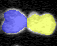
\includegraphics[width=\halfscalingfactor\textwidth]{images/joint/pipeline/78_merge_crop.png}
        };
        \node[inner sep=0,xshift=42,yshift=-42] (hyp_cc1) {
            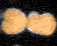
\includegraphics[width=\halfscalingfactor\textwidth]{images/joint/pipeline/78_cc_crop.png}
        };
    \end{scope}
    \begin{scope}[every node/.append style={yslant=0.5,xslant=-1},yslant=0.5,xslant=-1]
        \node[xshift=21,yshift=-21,inner sep=0] (hyp_cc2) {
            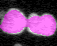
\includegraphics[width=\scalingfactor\textwidth]{images/joint/pipeline/79_cc_crop.png}
        };
    \end{scope}
    \coordinate (base1) at (merge1.north west |- cc2.south west);
    \coordinate (base2) at (cc1.south east |- cc2.south west);
    \draw [thick,
    black,decorate,decoration={brace,amplitude=10pt,mirror},xshift=0.4pt,yshift=-0.4pt]
    (base1) -- (base2) node[black,midway,yshift=-0.6cm]
    {Hypotheses Generation};
\end{scope}

%%% Local Variables: 
%%% mode: latex
%%% TeX-master: "../../../main"
%%% End: 
